\documentclass[xcolor=dvipsnames,compress,t,pdf,9pt]{beamer}
\input{template_presentation}
\usepackage{polyglossia}
\setdefaultlanguage{sanskrit}
\setotherlanguage{english}

\usepackage{fontspec}
\setmainfont{Segoe UI}

\newfontfamily\devanagarifont[Script=Devanagari]{Nakula}
\newfontfamily\devanagarifontsf[Script=Devanagari]{Nakula}
\newfontfamily\devanagarifonttt[Script=Devanagari]{Nakula}
\newfontfamily\devtransl[Mapping=DevRom]{Segoe UI}

\graphicspath{{images/}}
\title[\insertframenumber /\inserttotalframenumber]{YogaSutra Seminar 4: Vibhuti Pada — Experiences \& Powers}


\begin{document}

	\begin{frame}
	\titlepage
	\end{frame}

	\section[Intro]{Brief Introduction}
%%%%%%%%%%%%%%%%%%%%%%%%%%%%%%%%%%%%%%%%%%%%%%%%%%%%%%%%%%%%%%%%%%%%%%%%%%%%%%%%%%
\begin{frame}[fragile]\frametitle{Maharshi Patanjali महर्षि पतञ्जलि}

    \begin{columns}
    \begin{column}[t]{0.4\linewidth}
\begin{center}
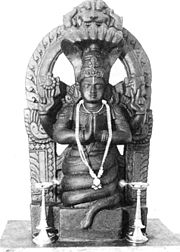
\includegraphics[width=0.5\linewidth,keepaspectratio]{images/yog15}
\end{center}
\begin{sanskrit}
योगेन चित्तस्य पदेन वाचां |
मलं शरीरस्य च वैद्यकेन |
योऽपाकरोक्तं प्रवरं मुनीनां |
पतञ्जलिं प्राञ्जलिरनतोस्मि ||
— राजा भर्तुहरि
\end{sanskrit}
    \end{column}
    \begin{column}[t]{0.6\linewidth}
        \begin{itemize}
        \item ``Father of Yoga''; lived approx.\ 200–500 BC
        \item Three legendary contributions:
            \begin{itemize}
            \item Purification of \textbf{mind} $\rightarrow$ \textbf{योगसूत्र}
            \item Purification of \textbf{speech} $\rightarrow$ महाभाष्य (Grammar)
            \item Purification of \textbf{body} $\rightarrow$ चरकसंहिता (Ayurveda, attributed)
            \end{itemize}
        \item Yoga existed before him; he \emph{systematized} and \emph{codified} it
        \item Not a new system:a living tradition organized into सूत्र (aphorisms)
        \end{itemize}
    \end{column}
  \end{columns}

\tiny{(Ref: Bhartuhari; Sadhguru on Patanjali)}

\end{frame}

%%%%%%%%%%%%%%%%%%%%%%%%%%%%%%%%%%%%%%%%%%%%%%%%%%%%%%%%%%%
\begin{frame}[fragile]\frametitle{Structure of Yoga Sutras:4 Chapters}

\begin{itemize}
\item \textbf{195/196 Sutras} arranged in 4 \textbf{पाद} (chapters/quarters)
\item सूत्र (sutra) = thread:minimum words, maximum meaning
\end{itemize}

\begin{center}
\begin{tabular}{|p{0.8cm}|p{3cm}|p{0.8cm}|p{2.4cm}|}
\hline
\textbf{Chapter} & \textbf{Name} & \textbf{Sutras} & \textbf{Theme} \\
\hline
1 & समाधिपाद Samadhi Pada & 51 & Concentration \\
2 & साधनपाद Sadhana Pada & 55 & Practice \\
3 & विभूतिपाद Vibhuti Pada & 56 & Experiences \\
4 & कैवल्यपाद Kaivalya Pada & 34 & Absolute Freedom \\
\hline
\end{tabular}
\end{center}

\begin{itemize}
\item Each chapter targets a different type of seeker and a different stage of the journey
\item Commentaries (भाष्य) starting with Vyasa are essential companions to the Sutras
\end{itemize}

\tiny{(Ref: Nancy Wile:Yoga Education Institute; पातंजल योग सूत्र)}

\end{frame}

%%%%%%%%%%%%%%%%%%%%%%%%%%%%%%%%%%%%%%%%%%%%%%%%%%%%%%%%%%%
\begin{frame}[fragile]\frametitle{Purpose:Three Core Principles}

The Yoga Sutras rest on three foundational principles (Nancy Wile):

\begin{enumerate}
\item \textbf{Suffering is internal}:not caused by outside forces but by our \emph{faulty perception} of ourselves and life. The situation is not the problem; our thoughts about the situation are.
\item \textbf{Peace is our true nature}:the unlimited, eternal peace we seek already exists within us, hidden by ignorance (\textbf{अविद्या}).
\item \textbf{Mastery of mind} = Self-Realization:only a single-pointed, calm mind can reveal the true Self (पुरुष).
\end{enumerate}

\vspace{3mm}
\begin{center}
{\large ``Yoga is not addition. It is subtraction:ceasing the compulsive activity of the mind.''}
\end{center}

\tiny{(Ref: Nancy Wile, Yoga Education Institute; Krishnamurthy Ramakrishnan)}

\end{frame}

%%%%%%%%%%%%%%%%%%%%%%%%%%%%%%%%%%%%%%%%%%%%%%%%%%%%%%%%%%%
\begin{frame}[fragile]\frametitle{Key Yogic Concepts}

\begin{itemize}
\item \textbf{पुरुष (Purusha)}:Pure consciousness; the Seer; eternal, unchanging
\item \textbf{प्रकृति (Prakriti)}:Primordial nature; source of all manifestation; made of three गुण
\item \textbf{चित्त (Chitta)}:Mind-stuff; four coordinated functions:
    \begin{itemize}
    \item \textbf{मनस्}:sensory receiver and motor director
    \item \textbf{बुद्धि}:intellect; discrimination and decision
    \item \textbf{अहंकार}:ego; the ``I-maker'' that claims ownership
    \item \textbf{चित्त}:memory store; repository of संस्कार (impressions)
    \end{itemize}
\item \textbf{वृत्ति (Vritti)}:modifications/ripples of the mind; the core problem Yoga addresses
\item \textbf{त्रिगुण (Triguna)}:three qualities of Prakriti: सत्व (clarity), रजस् (activity), तमस् (inertia)
\item \textbf{कैवल्य (Kaivalya)}:liberation; Purusha abiding in its own pure nature
\end{itemize}

\tiny{(Ref: Sankhya Darshana basis; Vyasa Bhashya)}

\end{frame}


\section[Vibhutipad]{Vibhuti Pada विभूतिपाद — Experiences \& Powers}
\input{yogsutra_vibhutipad}

\section[End]{Towards End}
%%%%%%%%%%%%%%%%%%%%%%%%%%%%%%%%%%%%%%%%%%%%%%%%%%%%%%%%%%%%%%%%%%%%%%%%%%%%%%%%%%
\begin{frame}[fragile]\frametitle{}
\begin{center}
{\Large References}
\end{center}
\end{frame}


%%%%%%%%%%%%%%%%%%%%%%%%%%%%%%%%%%%%%%%%%%%%%%%%%%%%%%%%%%%
\begin{frame}[fragile]\frametitle{References}

Many publicly available sources have been used in the preparation of this content. Some of the salient ones are listed below:

	\begin{itemize}
	\item Patanjali Yog Sutra https://patanjaliyogasutra.in/
	\item Yoga Sutra Study https://yogasutrastudy.info/
		\begin{itemize}
		\item [HA]: Hariharananda Aranya
		\item [IT]: I. K. Taimni
		\item [VH]: Vyasa Houston
		\item [BM]: Barbara Miller
		\item [SS]: Swami Satchidananda
		\item [SP]: Swami Prabhavananda
		\item [SV]: Swami Vivekananda
		\end{itemize}
	\item Prof. Edwin Bryant — \emph{The Yoga Sutras of Patanjali} (book + lectures)
	\item Dr. Ananda Balayogi Bhavanani — \emph{An Overview of the Yoga Sutras}, Integral Yoga Magazine
	\item Nancy Wile — \emph{The Yoga Sutras} (Yoga Teacher Training manual), Yoga Education Institute, 2014
	\item Krishnamurthy Ramakrishnan — \emph{Yoga Sutras for Daily Life}, LinkedIn Newsletter
	\item Wikipedia — \emph{Yoga Sutras of Patanjali}
	\item योग सूत्र का परिचय | Yoga Sutras of Patanjali | Yoga Sutras For QCI, UGC NET, Yoga All Exams - YouTube
	\item Patanjali Yoga Sutra Dr Mrudula Chaudhari
	\item Patanjali Yoga Sutras | Explanation by Anandmurti Gurumaa Gurumaa Ashram Verified
	\item Indica Course https://indica.courses/enroll/prof-m-a-narasimhan/maharshi-patanjali-yogasutras-learn-recite-ii/
	\item Swami J Patanjali Yoga Sutra https://swamij.com/yoga-sutras.htm
	\item Dr. Veena Londhe — \emph{An Introduction to Patanjali's Yoga Darshana}, Chinmaya Mission
	\end{itemize}

\end{frame}

%%%%%%%%%%%%%%%%%%%%%%%%%%%%%%%%%%%%%%%%%%%%%%%%%%%%%%%%%%%
\begin{frame}[fragile]\frametitle{Youtube Channels}



	\begin{itemize}
	\item Patanjali Yoga Sutras - English Yogic Gurukul - Anvita Dixit · Podcast
	\item Patanjali Yoga Sutras | Explanation by Anandmurti Gurumaa
	\item Complete Patanjali Yoga Sutras Chant with Meanings
	\item Patanjali Yoga Sutra Live Streams - The Sanskrit Channel
	\item The Sankrit Channel - "Detailed Patanjali Yoga Sutras with Pictures - Chapter 1-2-3-4"
	\end{itemize}

\end{frame}

%%%%%%%%%%%%%%%%%%%%%%%%%%%%%%%%%%%%%%%%%%%%%%%%%%%%%%%%%%%
\begin{frame}[fragile]\frametitle{}

\begin{center}
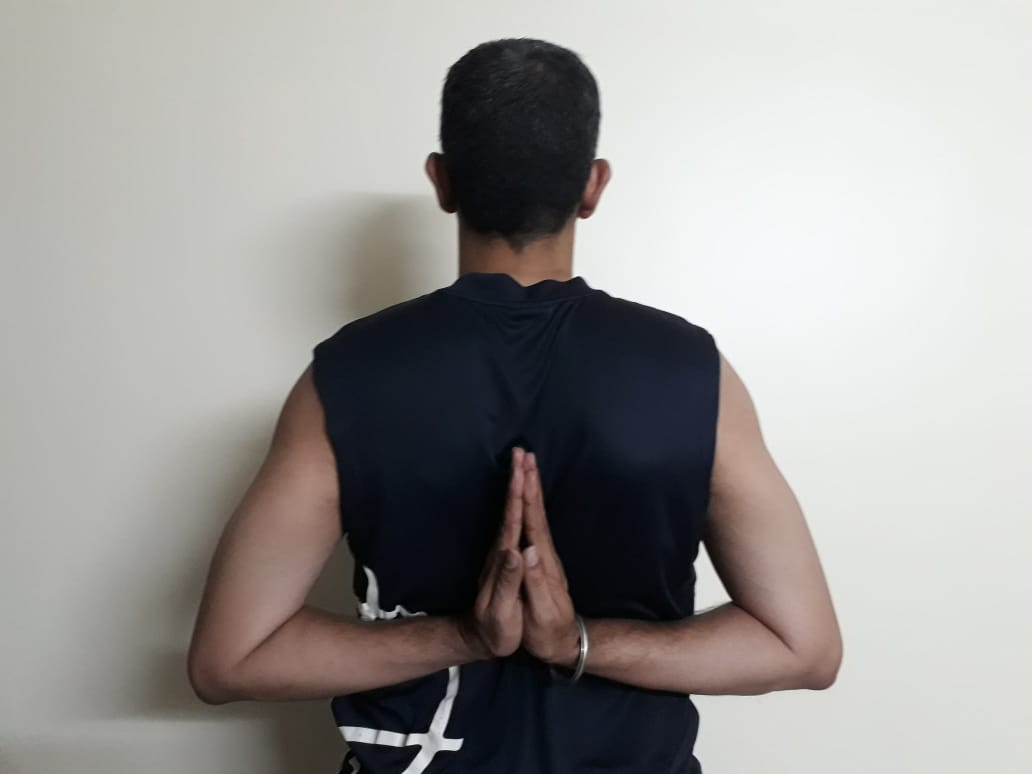
\includegraphics[width=0.8\linewidth,keepaspectratio]{my_yog_back}

Thanks धन्यवाद
\end{center}

\end{frame}



	\begin{frame}[c]{}
	Thanks ...
	\vspace{5mm}
	yogeshkulkarni@yahoo.com
	\end{frame}

\end{document}
